This section presents \NAME, a \emph{THRee-valued Integrated Verification Engine}. 
\NAME\ enriches an underlying three-valued model checker with a fully deductive verification approach.
%\footnote{\anna{The used procedure has been adapted from the one illustrated in~\cite{peled2001model} to be used with Kripke structures.}}

\setcounter{footnote}{0}

An overview of our proposal is presented in Figure~\ref{Fig.3vdv}.
\NAME\ provides the designer with two kinds of information: the model checking result and the deductive verification result.
The \emph{three-valued model checking} procedure presented in Section~\ref{sec:preliminaries} is used to verify whether the property $\phi$ of interest is definitely satisfied ($\LTLtrue$), possibly satisfied ($?$) or not satisfied ($\LTLfalse$) by the current partial model. 
If the property is \emph{not satisfied}, there exists some behavior which definitively violates the property of interest that does not depend on the unknown elements.
The model checker returns to the designer one of these behaviors, i.e., a definitive counterexample. 
Whenever a property is \emph{definitely satisfied}, its satisfaction does not depend on how the incomplete parts are refined.
Finally, if the property is \emph{possibly satisfied}, its satisfaction depends on how the uncertainty is removed.
The model checker returns a possible violating behavior.

\begin{figure}[b]
\begin{center}         
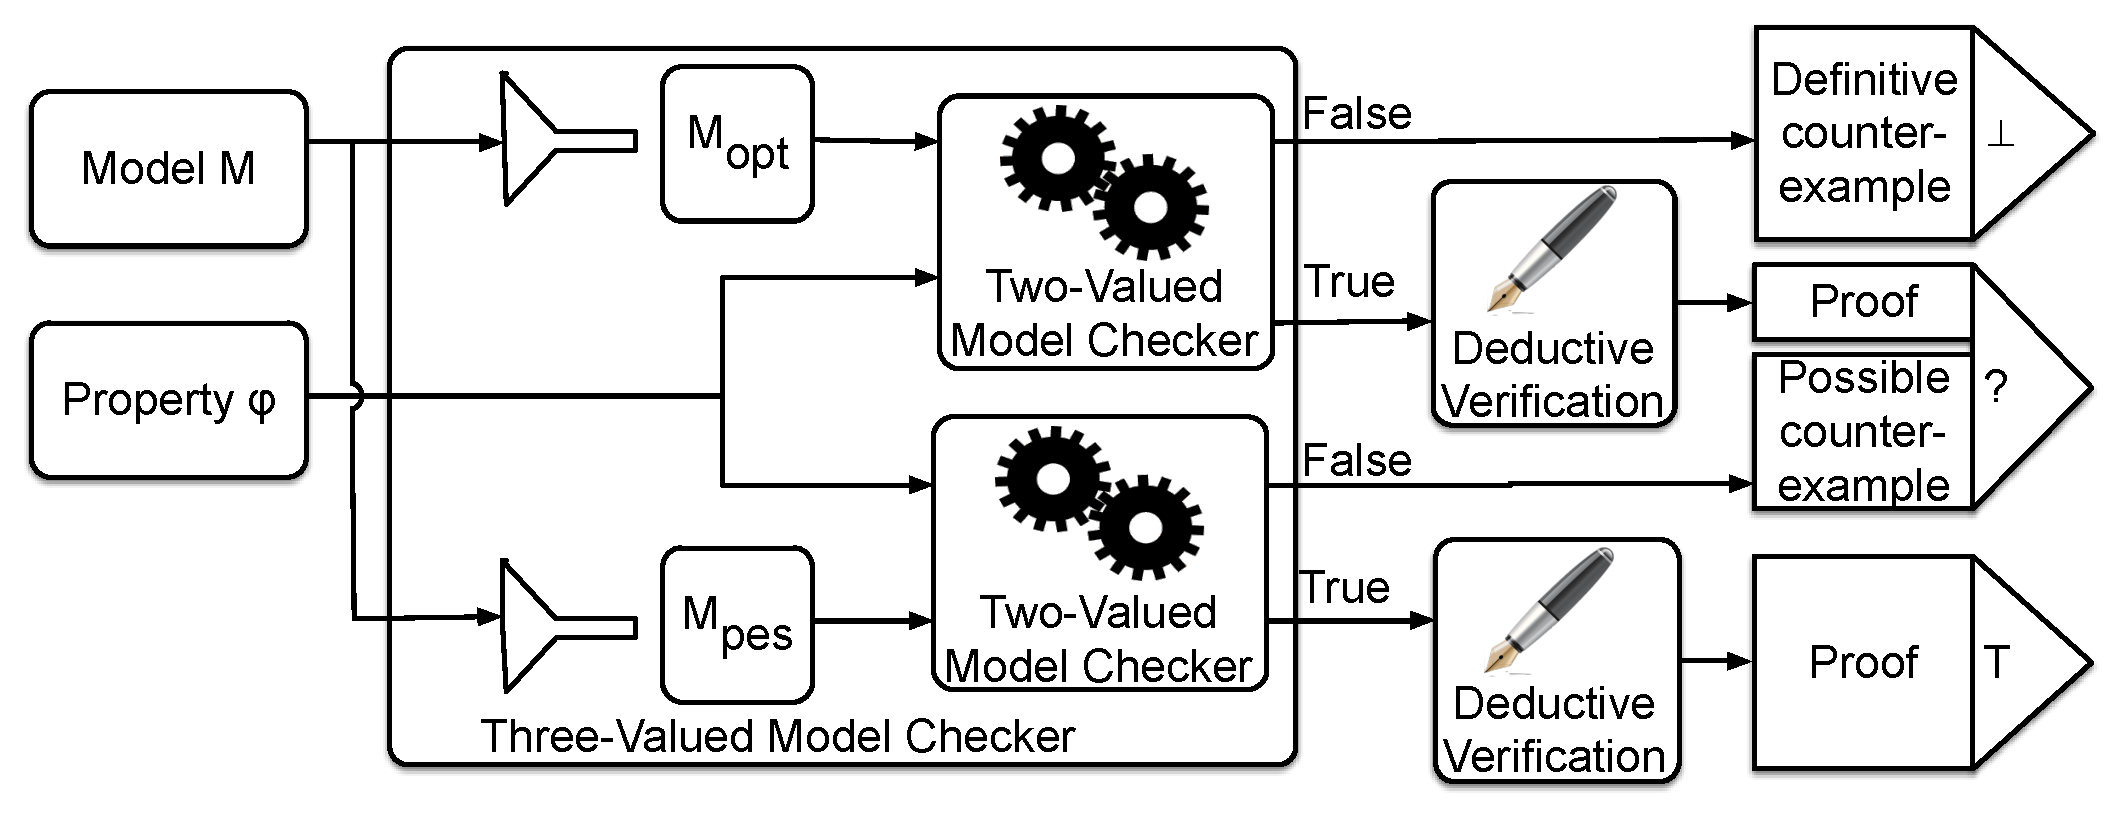
\includegraphics[width=9cm]{./images/atvaFig.pdf}
\end{center}
\caption{The proposed three-valued verification framework.}  
\label{Fig.3vdv}
\end{figure}

%Whenever the property is not satisfied a counterexample is returned. 
%The counterexample contains a path that violates the property of interest and does not depend on the $?$-propositions of $M$.

The \emph{deductive verification} engine is executed when a $\LTLtrue$ or $?$ value is returned by the model checker.
It is used to compute a proof which specifies explicitly why the property $\phi$ is definitely (possibly) satisfied by $M$, by incrementally adding logic assertions to the framework. 
When the automatic procedure is completed, the user obtains a proof that the system definitively/possibly satisfies the specification.
When a property is \emph{definitely satisfied}, the proof specifies to the designer why the search of a definitive/possible counterexample has failed.
Instead, whenever a property is \emph{possibly satisfied}, besides providing a possible counterexample, the proof specifies why a definitive counterexample has not been found.

%Finally, \remove{whenever} \anna{also when} the verification result is not conclusive \remove{($\bot$)}, the model checking algorithm returns a counterexample\remove{, which}\anna{. In this case it} specifies a possibly violating behavior by a possible complete model that refines the current incomplete model, which could be obtained by assigning specific values to the unknown propositions.  In addition, the \emph{deductive verification} framework\remove{, in this case,} provides a proof that the property is not false, i.e., $M$'s state space does not exhibit paths that violate $\phi$.


We instantiate \NAME\ considering PKSs and LTL formulae.
The deductive verification framework presented in Section~\ref{sec:theoremProving} is executed on the top of the three-valued model checker introduced in Section~\ref{sec:mcIncomplete}.
The extended version of the paper contains additional details on how these two frameworks are integrated. 
We discuss the correctness of \NAME\ w.r.t the three-valued and the thorough semantics.
We also analyze the behavior of the framework for a particular subset of LTL formulae called self-minimizing LTL formulae.
For clarification purposes, we summarize in Table~\ref{tab:results} the validity of the verification results obtained by the framework.

%In this work, we assume the model of the system to be specified using Partial Kripke Structures (PKSs)~\cite{bruns1999model} and we consider the properties of interest formalized using Linear Temporal Logic. 
%We also analyze the behavior of the framework for a particular subset of LTL formulae called self-minimizing LTL formulae, for which our framework obtains a meaningful result in all possible output cases.
%Both LTL and self-minimizing LTL formulae are considered w.r.t the three-valued LTL semantics and the thorough  semantics.
%For clarification purposes, we summarize in Table~\ref{tab:results} the validity of the verification results obtained by the framework when LTL and its subset are considered under the two discussed semantics.

%They can be identified using a set of syntactic constraints.
%Furthermore, for many LTL formulae, there exists a transformation, called semantic minimization, that transforms the formula into an equivalent self-minimizing LTL formula. 
%

\textbf{LTL formulae.} 
\emph{Three-valued LTL semantics.} 
When the three-valued model checker returns a $\LTLtrue$ value, no counterexample is returned.
By Proposition~\ref{def:mcImpliesGmc}, a property $\phi$  evaluated to $\LTLtrue$ considering the three-valued semantics, is also satisfied considering the thorough semantics.
Consequently, this case corresponds to a correct verification and it is marked with a \validCounterexample\ symbol in Table~\ref{tab:results}.
In these cases, \NAME\ uses the deductive verification framework to prove that $\phi$ is satisfied.
Since this property also holds considering the thorough semantics, the proof is \emph{valid} and demonstrates that any completion of $M$ satisfies $\phi$. 
The cases in which \NAME\ generates valid proofs are marked with a \validProof\ symbol.

When the model checker returns a $\LTLfalse$ value, the counterexample shows to the designer a behavior that violates the property of interest.
By Proposition~\ref{def:mcImpliesGmc}, a property $\phi$  evaluated to $\LTLfalse$ considering the three-valued semantics, is also not satisfied considering the thorough semantics.
Thus, the counterexample is a valid counterexample that proves the existence of a completion of $M$ that violates $\phi$.
For this reason, this case is marked with a \validCounterexample\ symbol in Table~\ref{tab:results}.
 
 As specified in Section~\ref{sec:mcIncomplete}, the three-valued model checker returns a $?$ value more often than expected: there are cases in which a $?$ is returned but all the completions of the model either satisfy or do not satisfy the property of interest. 
In this case, the counterexample can be a spurious counterexample, i.e., not valid under the thorough semantics.
We indicate the case in which a spurious counterexample can be found with the \spuriosCounterexample\ symbol.
Since when a property $\phi$ is evaluated to $?$ there could exist a completion that violates $\phi$, the produced proof cannot be considered valid under the thorough semantics.
We indicate the case in which it is possible to generate such a proof with the \notvalidProof\ symbol.

\begin{table}[t]
\centering
\caption{LTL and self-minimizing LTL validity of the framework outputs.}
\label{tab:results}
\begin{tabular}{   c  c | c | c | c | c |}
\cline{3-6}
 & & \multicolumn{2}{c |}{LTL} &    \multicolumn{2}{c |}{Self-minimizing LTL} \\
\cline{1-6}
  \multicolumn{1}{| c }{Result} & \multicolumn{1}{| c }{Type of Output} & \multicolumn{1}{| c |}{Three-valued} & Thorough & Three-valued & Thorough\\
\cline{1-6} 
  \multicolumn{1}{| c }{\multirow{2}{*}{$\LTLtrue$}} &  \multicolumn{1}{| c }{Verification result} & \multicolumn{1}{| c |}{\validCounterexample} & \validCounterexample & \validCounterexample &  \validCounterexample \\
    \cline{2-6}
 \multicolumn{1}{| c }{} &  \multicolumn{1}{| c }{Proof} & \multicolumn{1}{| c |}{\validProof} & \validProof & \validProof & \validProof \\
  \cline{1-6}
  \multicolumn{1}{| c }{\multirow{2}{*}{$?$}} &  \multicolumn{1}{| c }{Possible counterexample} & \multicolumn{1}{| c |}{\spuriosCounterexample} & $\boldsymbol{-}$ & \validCounterexample & \validCounterexample \\
  \cline{2-6}
  \multicolumn{1}{| c }{} &  \multicolumn{1}{| c }{Proof} &\multicolumn{1}{| c |}{\notvalidProof} & $\boldsymbol{-}$ & \validProof & \validProof \\

   \cline{1-6}
 \multicolumn{1}{| c }{$\LTLfalse$} & \multicolumn{1}{| c }{Definitive counterexample} &  \multicolumn{1}{| c |}{\validCounterexample} & \validCounterexample & \validCounterexample & \validCounterexample  \\
 \hline
\end{tabular}
\end{table}

\emph{Thorough LTL semantics.} As previously discussed, whenever a $\LTLtrue$ ($\LTLfalse$) result is returned by the three-valued model checker, the result is valid also under the thorough semantics.
For this reason, \NAME\ can be successfully applied in these cases.
Moreover, when the three-valued model checker returns a $?$ value, the result can be not valid. 
In this case, if a correct result is required, the use of a generalized model checking procedure~\cite{bruns2000model} (not discussed here) becomes necessary. 
Consequently, a more generic deductive verification framework, developed on top of the generalized model checking procedure, should be used.
In Table~\ref{tab:results} this case is marked with a $\boldsymbol{-}$ symbol, since currently \NAME\ does not support it.


\textbf{Self-minimizing LTL formulae.} 
Self-minimizing LTL formulae are a subset of LTL formulae that present a really interesting property: the three-valued and the thorough semantics coincide, i.e., if $\phi$ is self-minimizing, then $[(M, s) \models \phi]=[(M, s) \models \phi]_t$.
Therefore, the three-valued model checking framework presented in Section~\ref{sec:mcIncomplete} can also be used to verify a property under the thorough semantics. 
For this reason, in Table~\ref{tab:results}, the cells associated with the three-valued model checking procedure are marked with \validCounterexample.
Whenever the three-valued model checker returns $\LTLtrue$, Proposition~\ref{def:self-minimizing} certifies that the proof is valid also under the thorough semantics. 
Moreover, if $?$ is returned, the proof demonstrates that a definitive counterexample cannot be found.
For this reason, in Table~\ref{tab:results}, the cells associated with the deductive verification procedure are marked with \validProof.

%\begin{theorem}(The verification procedure is correct)
%\end{theorem}
%\begin{proof}
%
%Since $\phi$ is a self-minimizing temporal logic formula, if the model $M$ violates the formula there must exist a path in the optimistic approximation $M_o$ which does not satisfy the formula $\phi$.
%By providing the developer with a proof that $M_o$ does not violate $\phi$ we are formally justifying \emph{why} the property is not definitely violated in $M$.
%Furthermore, since  $\phi$ is a self-minimizing temporal logic formula, if the model $M$ possibly violates the formula, there must exist a path in the pessimistic approximation $M_p$ which does not satisfy the formula $\phi$.
%If such a path is not found, by proving that $M_p$ satisfies $\phi$ we are proving to the developer that every assignment to the unknown atomic propositions makes $\phi$ definitely satisfied.
%\end{proof}

%\vspace{-0.6cm}



